\section{New Design}

The WWLLN service unit was redesigned due to the obsolescence of the previous Trimble GPS unit, this redesign allowed for several other major revisions to the board:

\begin{itemize}
\item{Built in USB-Serial conversion}
\item{On board computer}
\item{Remote controlled pre-amp power system}
\item{Remove inline preamp LEDs}
\item{Increased stereo driving power}
\item{Two-way GPS serial communication}
\end{itemize}

The biggest change is the addition of the onboard computer, eliminating the need for a separate CPU to be installed with every service unit.
The Gumstix WaterStormCOM with Tobi breakout board was chosen for the onboard computer.
An on board computer is able to toggle the preamp power supply remotely, communicate with the GPS engine via TSIP, and standardize the host computer capabilities.
The USB-serial convert is used to output GPS messages to an external computer if desired, and two communication can be switched from the GPS to the USB port via the use of an onboard jumper.
Finally the system is designed to be operated remotely via SSH, but it does have the ability to use a keyboard, mouse and monitor through a powered USB hub and HDMI capable display.

\section{Gumstix Selection}

There are a few important aspects of the Gumstix WaterStormCOM that makes it suitable as a WWLLN service unit computer.
Other compact computers meet most, if not all, of these requirements and they should be satistifed for future upgrades and revisions to the design.
The primary requirements are:

\begin{itemize}
\item{48~kHz stereo input}
\item{Ethernet connection}
\item{Linux OS}
\end{itemize}

Once these are met the secondary requirements are:

\begin{itemize}
\item{Serial input (GPS comminication)}
\item{8~GB of memory}
\item{512~MB of RAM}
\item{USB}
\item{Video out (VGA/DVI/HDMI)}
\item{Low power ($<1$ A)}
\item{Low cost ($<$\$300)}
\end{itemize}

Other alternative systems include BeagleBoards, PandaBoard, Gumstix (other models), and maybe future versions of RaspberryPi.
One consideration not listed above is size.
The Gumstix was chosen for the final computer since it could fit into the previous form factor for the service units, other systems such as BeagleBoards were too large to fit easily.

Another important note is that some of the requirements can be remedied with USB peripherals if suitable ones are found.
RaspberryPi with a USB soundcard could work in lieu of the Gumstix, however no USB soundcard could be reliable found that accurately processed the GPS pulse per second signal.

\section{Layout and Design}

The Eagle files (v5) are available on flash5 at /home/mlhutch/eagle/ or through a git repository (see Appendix~\ref{thesis:appendix:code}. 

\subsection{Design}

The board design is shown in Figure~\ref{su:fig:suSchematic} with corresponding component names and values.
The Gumstix is represented as a 40 pin header and a matching header needs to be soldered to the Tobi breakout board.
One adjustment that may need to be changed in future iterations is the voltage divider on the VLF and PPS signal output to the internal stereo jack (upper left of diagram).
Current values are set to reduce the two signals to within the input voltages of the Gumstix sound card.

\begin{figure}[ht!]
   \centering
   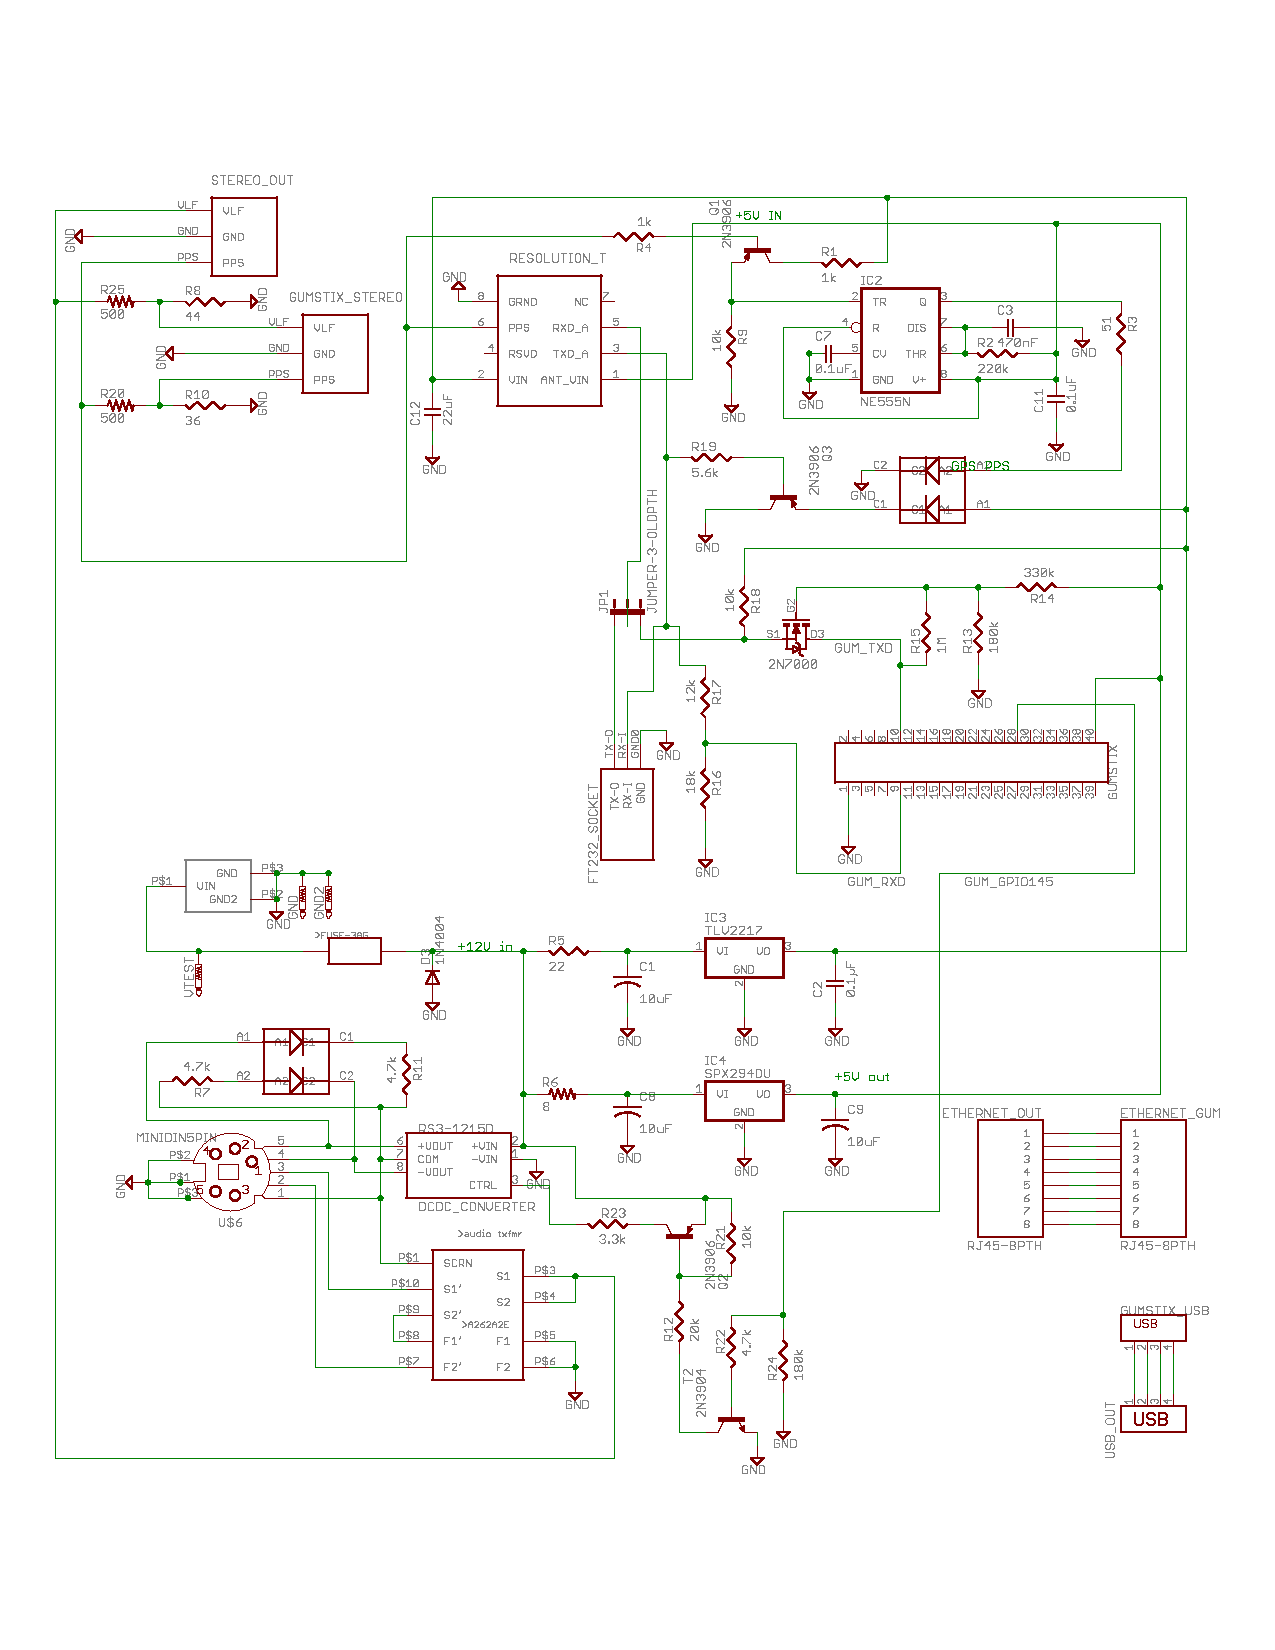
\includegraphics[scale=.75]{Appendix/Figures/wwlln_SU_v4_Schematic.pdf} 
   \caption{WWLLN Service Unit v4d design.}
   \label{su:fig:suSchematic}
\end{figure}

\subsection{Layout}

Unlike previous versions of the service unit most small components (resistors, capacitors, etc.) are placed on the underside of the board so the same form factor can be used.
The overall layout is shown in Figure~\ref{su:fig:suBoard} with the topside in Figure~\ref{su:fig:suTop} and bottom in Figure~\ref{su:fig:suBot}.
For heating issues the two voltage regulators need to be screwed onto the board with metal screws which act as heat sinks and connect them to the ground plane for heat dissipation.
Both the USB and ethernet jacks are on the board so the Gumstix does not face directly out of the box, preventing inevitable wear and tear on the Gumstix itself.
The HDMI plug is not on the board due to the inability to wire two jacks together (pins are spaced too close) so a wall-mount HMDI extension cord is used instead.

\begin{figure}[ht!]
   \centering
   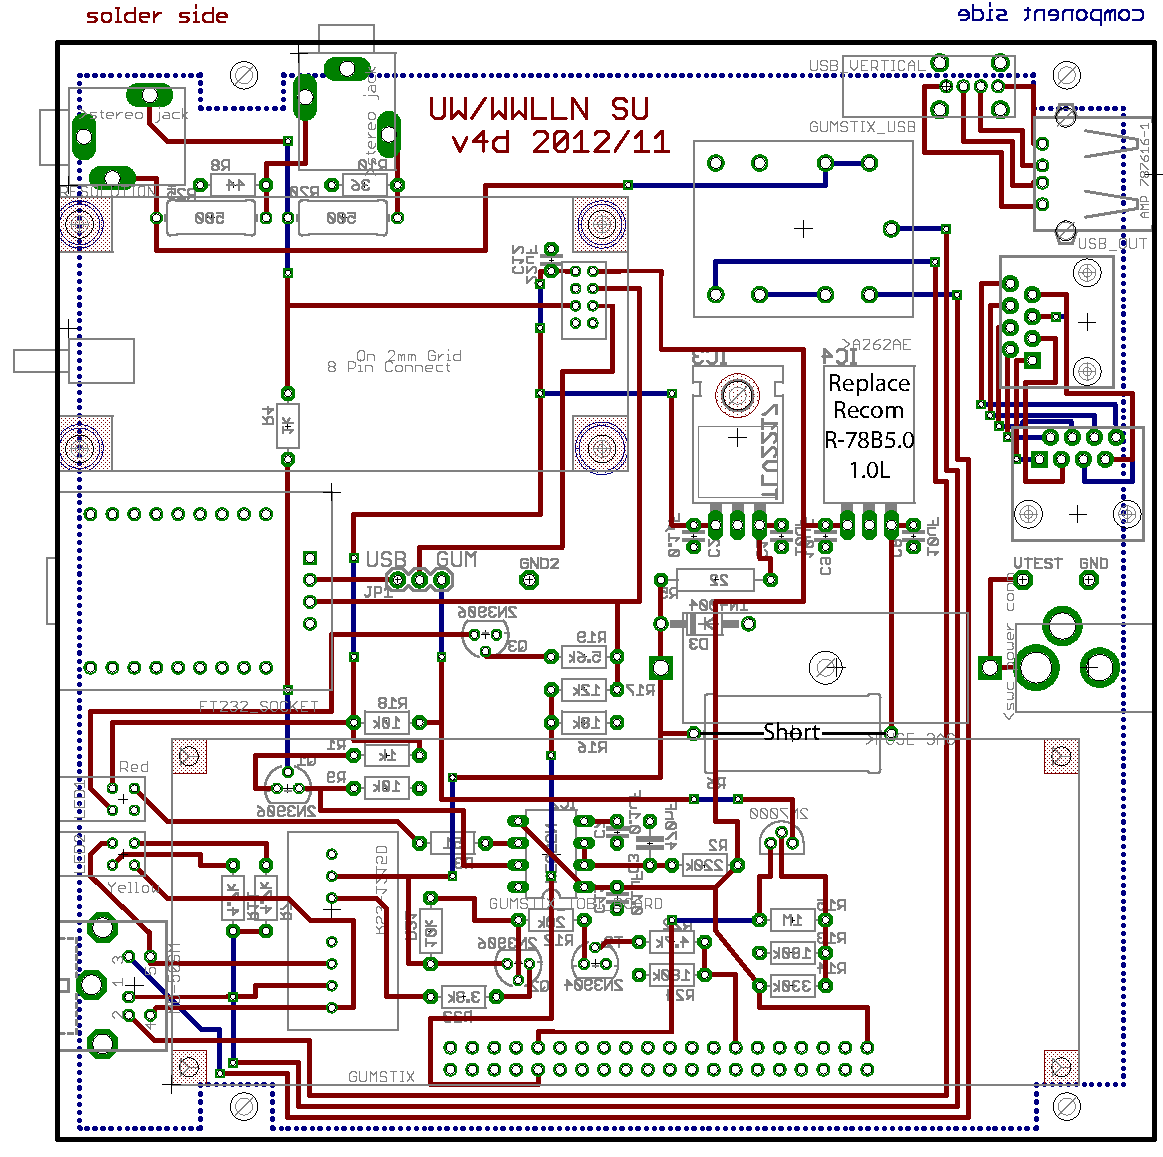
\includegraphics[scale=.75]{Appendix/Figures/wwlln_SU_v4.pdf} 
   \caption{WWLLN Service Unit v4d Schematic}
   \label{su:fig:suBoard}
\end{figure}

\begin{figure}[ht!]
   \centering
   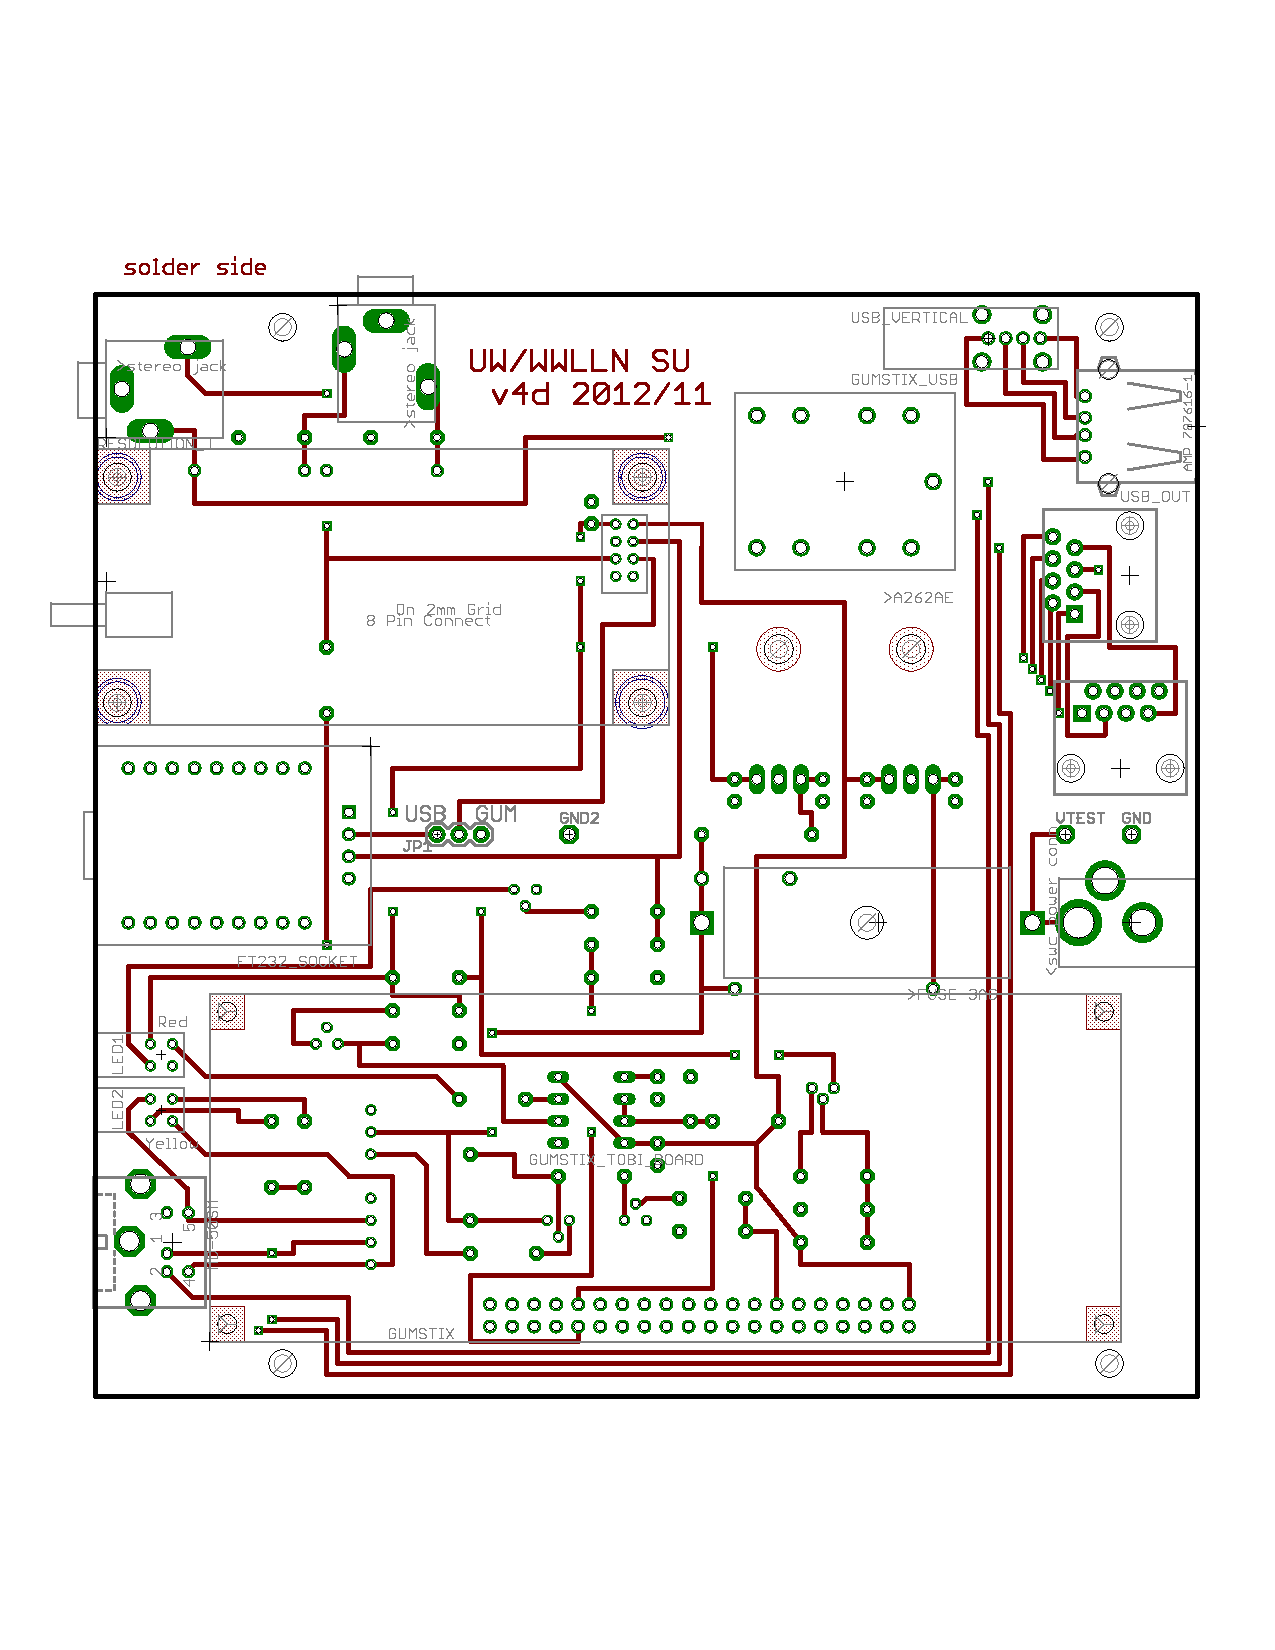
\includegraphics[scale=.75]{Appendix/Figures/wwlln_SU_v4_top.pdf} 
   \caption{WWLLN Service Unit v4d Topside}
   \label{su:fig:suTop}
\end{figure}

\begin{figure}[ht!]
   \centering
   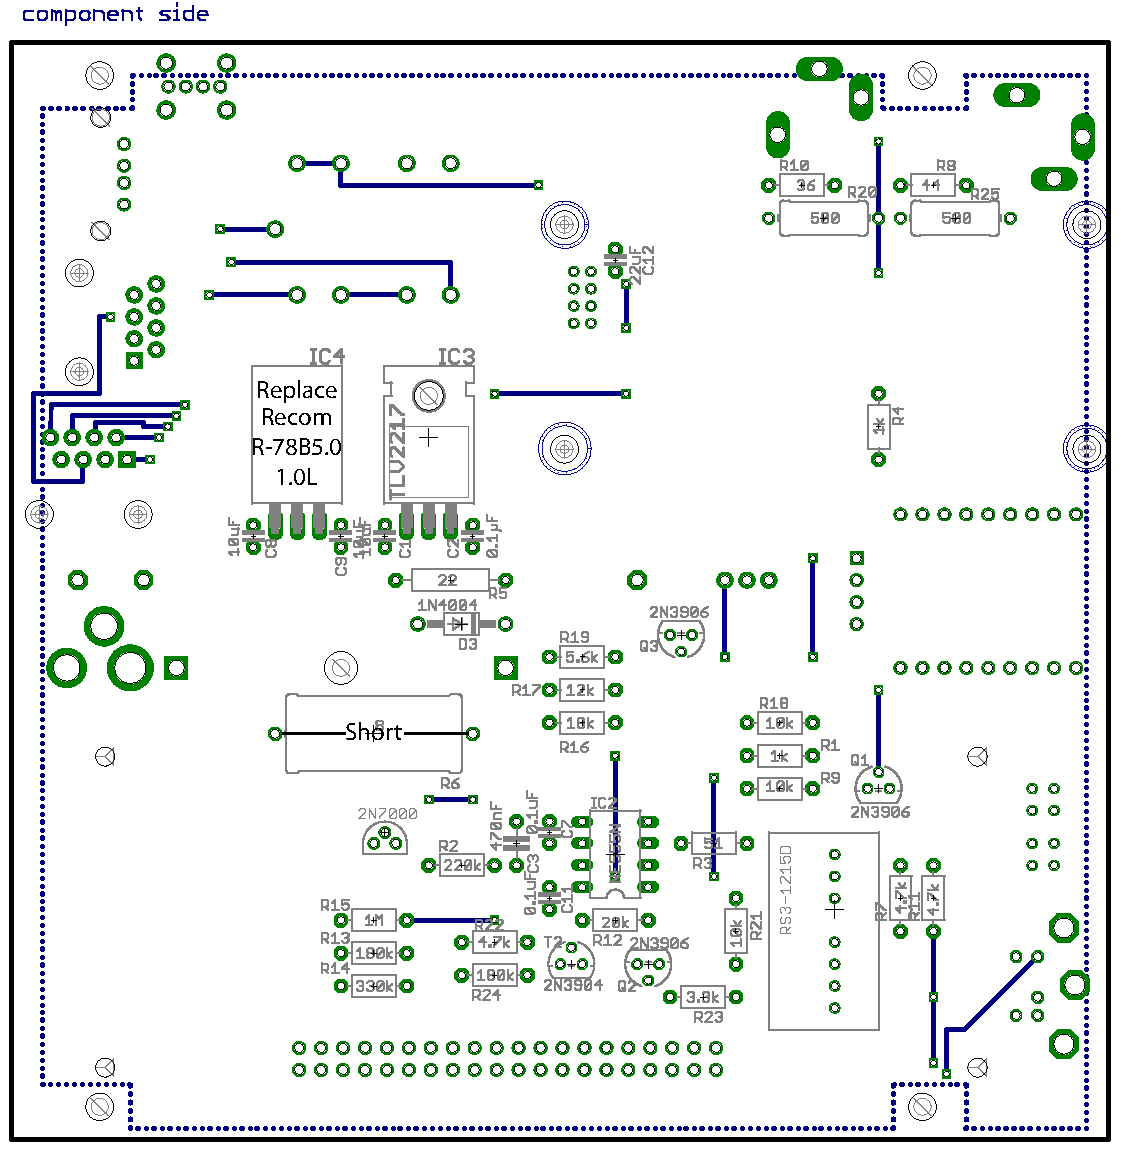
\includegraphics[scale=.75]{Appendix/Figures/wwlln_SU_v4_bottom.pdf} 
   \caption{WWLLN Service Unit v4d Bottomside}
   \label{su:fig:suBot}
\end{figure}

\section{Parts List}

The most recent parts list for the entire service unit, including price estimates are given in Table~\ref{su:table:suPrice}.
Total price for the service unit, excluding external cables and connectors, is \$546 before shipping and tax.
Price breaks are available for many of the components which can bring down the total price.

\begin{landscape}
\begin{center}
\begin{longtable}{|p{2in}|p{1.5in}|p{.75in}|p{.5in}|p{.5in}|p{1in}|p{1.5in}|}
\caption{WWLLN Service Unit Parts List (2013/02/19)}\\
\label{su:table:suPrice}\\
\hline
\bf Part & \bf Value & \bf Quantity  & \bf Unit Price & \bf Price & \bf Supplier & \bf Part Number\\ 
\hline
\endfirsthead
\multicolumn{4}{c}
{\tablename\ \thetable\ -- \textit{Continued from previous page}} \\
\hline
\bf Part & \bf Value & \bf Quantity  & \bf Unit Price & \bf Price & \bf Supplier & \bf Part Number\\ 
\hline
\endhead
\hline \multicolumn{4}{r}{\textit{Continued on next page}} \\
\endfoot
\hline
\endlastfoot
Part & Value & Quantity  & Unit Price & Price (SU) & Supplier & Part Number\\ 
Service Units &  & 5 & 545.632 &  &  & \\ 
HDMI Cable (1.5') & Panel Mount 3' Cable & 1 & 11.67 & 11.67 & Amazon & \\ 
MicroSD Card & SanDisk 16GB microSDHC & 1 & 9.5 & 9.5 & Amazon.com & \\ 
Stereo Cable (1', Right Angle) &  & 1 & 4.83 & 4.83 & Amazon.com & \\ 
2-56 Nuts &  & 4 & 0.1055 & 0.422 & Digikey & H612-ND\\ 
2-56 Screws (.75") &  & 4 & 0.0732 & 0.2928 & Digikey & H702-ND\\ 
2-56 Standoff (.375") &  & 4 & 0.82 & 3.28 & Digikey & 1797DK-ND\\ 
2-56 Washer &  & 8 & 0.053 & 0.424 & Digikey & 3357K-ND\\ 
3.3V Regulator & TLV2217 & 1 & 0.98 & 0.98 & Digikey & 296-21611-5-ND\\ 
4-40 Nuts &  & 18 & 0.0149 & 0.2682 & Digikey & H216-ND\\ 
4-40 Screws (.75") &  & 10 & 0.0285 & 0.285 & Digikey & H350-ND\\ 
4-40 Standoffs (.25") &  & 4 & 0.62 & 2.48 & Digikey & 1902AK-ND\\ 
4-40 Standoffs (.75") &  & 4 & 0.98 & 3.92 & Digikey & 8440EK-ND\\ 
555 Timer & NE555N & 1 & 0.42 & 0.42 & Digikey & 497-1963-5-ND\\ 
Box & L190-ND & 1 & 20 & 20 & Digikey & L190-ND\\ 
Capacitor 470nF & 470nF & 1 & 0.29 & 0.29 & Digikey & 445-5301-ND\\ 
Capacitor 0.1uF & 0.1uF & 3 & 0.33 & 0.99 & Digikey & 490-3810-ND\\ 
Capacitor 22uF & 22uF & 1 & 0.95 & 0.95 & Digikey & 478-1875-ND\\ 
Capacitor 10uF & 10uF & 3 & 0.81 & 2.43 & Digikey & 478-1839-ND\\ 
DCDC Converter (15V) & RS3-1215D & 1 & 20.58 & 20.58 & Digikey & 945-1565-5-ND\\ 
Diode & 1N4004 & 1 & 0.25 & 0.25 & Digikey & 1N4004-TPMSCT-ND\\ 
Ethernet Socket & RJ45-8PTH & 1 & 1.37 & 1.37 & Digikey & A31442-ND\\ 
Ethernet Socket (Vertical) & 380-1050-ND & 1 & 1.29 & 3.22 & Digikey & 380-1050-ND\\ 
Pins (M-M) & FT-232 and Jumper & 1 & 2.17 & 2.17 & Digikey & 929834E-03-36-ND\\ 
Fuse Socket & FUSE-3AG & 1 & 1.19 & 1.19 & Digikey & F1498-ND\\ 
Fuses & F2508-ND & 3 & 0.38 & 1.14 & Digikey & F2508-ND\\ 
Gumstix Battery & ML-621S/ZTN & 1 & 1.78 & 1.78 & Digikey & P007-ND\\ 
Gumstix Header & 40 pin header & 1 & 2.18 & 2.18 & Digikey & S9200-ND\\ 
Gumstix Socket & 40 pin mount & 1 & 0.86 & 0.86 & Digikey & S9175-ND\\ 
Jumper & S9338-ND & 1 & 0.11 & 0.11 & Digikey & S9338-ND\\ 
LED Red & LED4 & 1 & 1.23 & 1.23 & Digikey & 67-1254-ND\\ 
LED Yellow & LED4 & 1 & 1.22 & 1.22 & Digikey & 67-1256-ND\\ 
Minidin 5-pin & MINIDIN5PIN & 1 & 1.53 & 1.53 & Digikey & CP-2250-ND\\ 
Transistor MOSFET & 2N7000 & 1 & 0.39 & 0.39 & Digikey & 2N7000\_D26ZCT-ND\\ 
Transistor NPN & 2N3904 & 1 & 0.42 & 0.42 & Digikey & 2N3904-APCT-ND\\ 
Transistor PNP & 2N3906 & 3 & 0.42 & 1.26 & Digikey & 2N3906-APCT-ND\\ 
Power Jack & BARREL\_POWER\_CONN & 1 & 1.52 & 1.52 & Digikey & SC1313-ND\\ 
Resistor 8 & 8 (5W rated) & 1 & 0.55 & 0.55 & Digikey & 8.2W-5-ND\\ 
Resistor 22 & 22 (1 W rated) & 1 & 0.14 & 0.14 & Digikey & 22WCT-ND\\ 
Resistor 44 & 44 & 1 & 0.09 & 0.09 & Digikey & CF18JT43R0CT-ND\\ 
Resistor 51 & 51 & 1 & 0.09 & 0.09 & Digikey & CF18JT51R0CT-ND\\ 
Resistor 36 & 36 & 1 & 0.09 & 0.09 & Digikey & CF18JT36R0CT-ND\\ 
Resistor 500 & 500 & 2 & 0.97 & 1.94 & Digikey & PPC1D500CT-ND\\ 
Resistor 1k & 1k & 2 & 0.09 & 0.18 & Digikey & CF18JT1K00CT-ND\\ 
Resistor 3.3k & 3.3k & 1 & 0.09 & 0.09 & Digikey & CF18JT3K30CT-ND\\ 
Resistor 4.7k & 4.7k & 3 & 0.09 & 0.27 & Digikey & CF18JT4K70CT-ND\\ 
Resistor 5.6k & 5.6k & 1 & 0.09 & 0.09 & Digikey & CF18JT5K60CT-ND\\ 
Resistor 10k & 10k & 3 & 0.09 & 0.27 & Digikey & CF18JT10K0CT-ND\\ 
Resistor 12k & 12k & 1 & 0.09 & 0.09 & Digikey & CF18JT12K0CT-ND\\ 
Resistor 18k & 18k & 1 & 0.09 & 0.09 & Digikey & CF18JT18K0CT-ND\\ 
Resistor 20k & 20k & 1 & 0.09 & 0.09 & Digikey & CF18JT20K0CT-ND\\ 
Resistor 180k & 180k & 2 & 0.09 & 0.18 & Digikey & CF18JT180KCT-ND\\ 
Resistor 220k & 220k & 1 & 0.09 & 0.09 & Digikey & CF18JT220KCT-ND\\ 
Resistor 330k & 330k & 1 & 0.09 & 0.09 & Digikey & CF18JT330KCT-ND\\ 
Resistor 1M & 1M & 1 & 0.09 & 0.09 & Digikey & CF18JT1M00CT-ND\\ 
Resolution T Socket & 8 pin 2mm pitch & 1 & 1.06 & 1.06 & Digikey & H10922-ND\\ 
Stereo Jack & PHONO\_STEREO & 2 & 1.8 & 3.6 & Digikey & SC1465-ND\\ 
USB A Jack & USB-787616 & 1 & 1.44 & 1.44 & Digikey & A31726-ND\\ 
USB A Jack (Angled) & ED2991-ND & 1 & 0.64 & 0.64 & Digikey & ED2991-ND\\ 
USB-Serial Socket & 929974E-01-36-ND & 1 & 2.57 & 2.57 & Digikey & 929974E-01-36-ND\\ 
Gumstix Expansion Board & Tobi & 1 & 69 & 69 & Gumstix & \\ 
Gustix COM & WaterSTORM & 1 & 169 & 169 & Gumstix & \\ 
Ethernet Cable (2') & 3421 & 1 & 0.92 & 0.92 & Monoprice & 3421\\ 
USB Cable & 1.5' A-A Cable & 1 & 0.85 & 0.85 & Monoprice & 8609\\ 
5V Regulator & SPX2940U & 1 & 1.75 & 1.75 & Mouser & 701-SPX2940U-L-5-0\\ 
A262A2E Enclosure & A262CAN & 1 & 7.78 & 7.78 & Newark & 25M7635\\ 
Audio Transformer & A262A2E & 1 & 16.7 & 16.7 & Newark & 02M8356\\ 
USB-Serial FT232RL & Bob-00718 & 1 & 14.95 & 14.95 & Sparkfun & BOB-00718\\ 
Board Fabrication & Sunstone Prototype Board & 1 & 80 & 80 & Sunstone & \\ 
RESOLUTION\_T & RESOLUTION\_T & 1 & 65 & 65 & Trimble & 
\end{longtable}
\end{center}
\end{landscape}

\section{Construction}

Service unit construction steps:

\begin{enumerate}
\item{Populate board with components}
\item{Add in socket for USB-Serial converter}
\item{Add in pins for GPS jumper}
\item{Add jumper set to Gumstix}
\item{Screw down voltage regulators}
\item{Solder connection pins to USB-serial converter}
\item{Solder matching header to Gumstix Tobi board (with COM detached!)}
\item{Test board (see Section~\ref{su:subsection:suTest1})}
\item{Mount GPS and USB-serial converter}
\item{Test board (see Section~\ref{su:subsection:suTest2})}
\item{Mount Gumstix to board}
\item{Plug USB, ethernet, HDMI, and stereo cables into Gumstix}
\item{Plug USB, ethernet, and stereo into Service Unit board}
\item{Insert formatted microSD card into Gumstix board}
\item{Test board and Gumstix (see Section~\ref{su:subsection:suTest3})}
\item{Drill out holes in Service Unit box (Figures~\ref{su:fig:suBox} and~\ref{su:fig:suBoxBot})}
\item{Attach HDMI wall mount to side of box}
\item{Mount Service Unit board into box and wrap cables to fit}
\item{Final Service Unit and Gumstix test (see Section~\ref{su:subsection:suTest4})}
\end{enumerate}

\begin{landscape}
\begin{figure}[ht!]
   \centering
   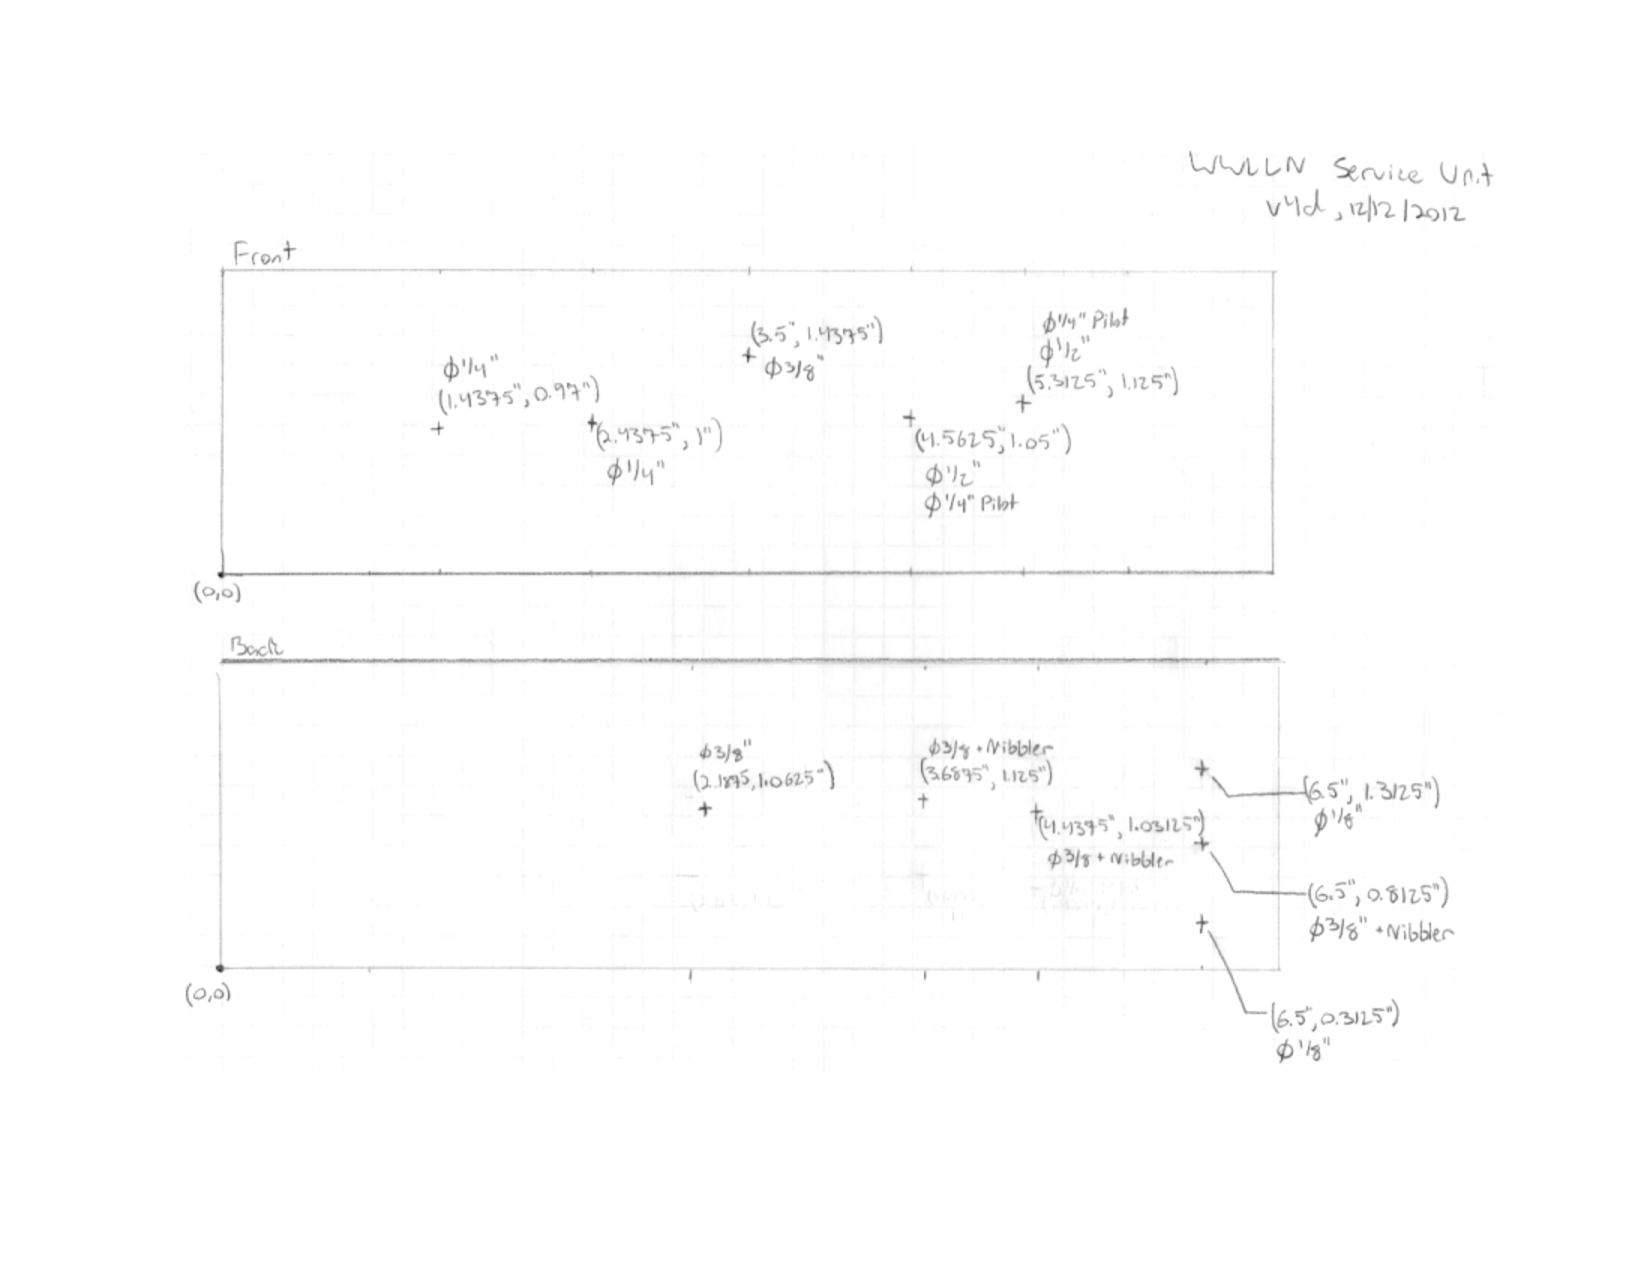
\includegraphics[scale=1]{Appendix/Figures/su_box_holes_sides.pdf} 
   \caption{Schematic for Service Unit box holes.}
   \label{su:fig:suBox}
\end{figure}
\end{landscape}

\begin{landscape}
\begin{figure}[ht!]
   \centering
   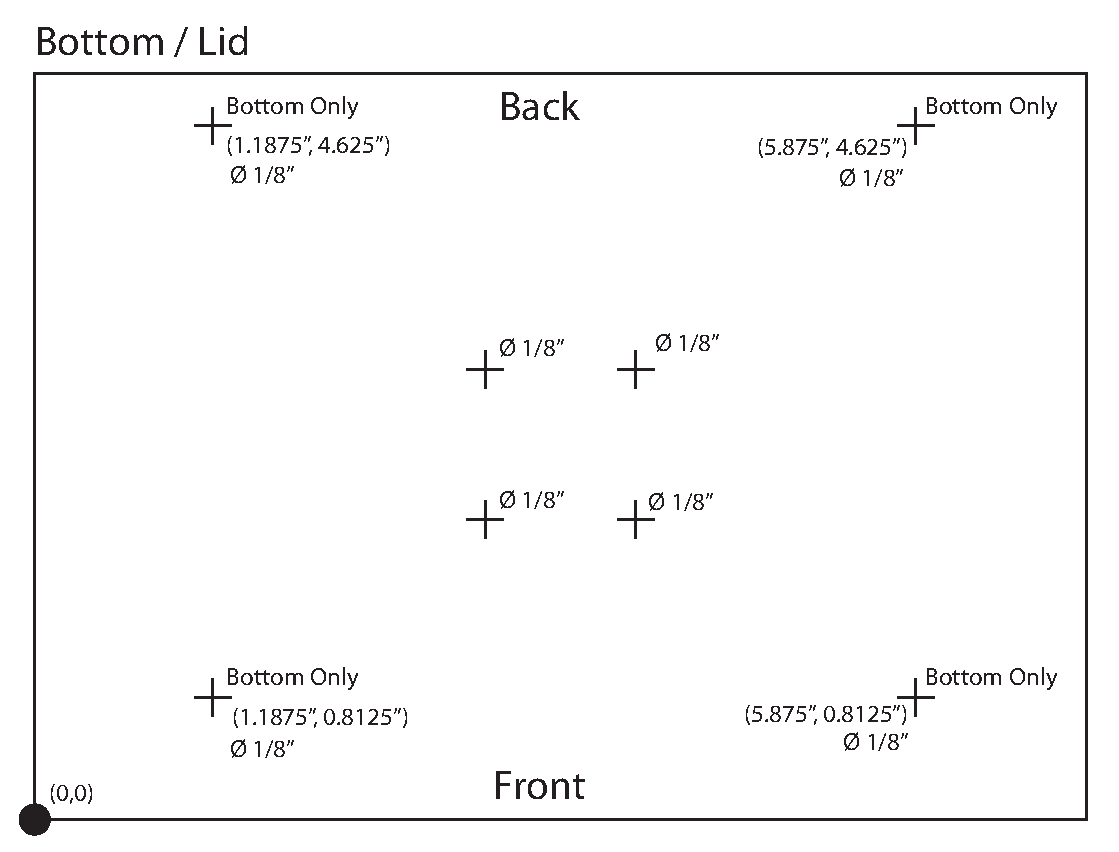
\includegraphics[scale=1]{Appendix/Figures/su_box_holes_bottom.pdf} 
   \caption{Schematic for Service Unit mounting holes.}
   \label{su:fig:suBoxBot}
\end{figure}
\end{landscape}

\section{Testing Procedures}

\subsection{Initial Board Test}
\label{su:subsection:suTest1}

Without an external boards (Gumstix, GPS, etc) connected slowly raise the input voltage from 0 to 12~V. 
At 12~V the board should be drawing near to 120~mA, and both yellow LEDs should be on.
The yellow LEDs indicate that the preamp power supply defaults on without the Gumstix plugged in.
Test the voltages for the GPS and Gumstx mounts.
The GPS should have two voltages, 5~V on pin 1 and 3.3~V on pin 2, all other pins should be 0~V.
If the USB-serial jumper it set to Gumstix, then the GPS will have a voltage on pin 5.
The Gumstix socket should have 0~V everywhere except on pin 40 which should be 5~V and pin 10 which should be 0.8~V.

\subsection{GPS Power Test}
\label{su:subsection:suTest2}

Turn off the board and plug in the GPS engine.
At 12~V power the board should be drawing 240~mA.
The bottom red LED should be blinking and the top one should be on.

\subsection{Gumstix Power Test}
\label{su:subsection:suTest3}

Plug in to the Gumstix and connect the ethernet (the ethernet LEDs allow for a quick check of the system).
Power the GPS with a 12~VDC wall plug, not a variable power supply.
During the Gumstix startup it draws near to 1~A briefly which can cause a drop in voltage with a variable power supply, this restarting the Gumstix.
After about 30 seconds the ethernet lights should start to blink and flash on the Gumstix ethernet port, indicating it has booted fully.
While idling the board should be drawing 600-700~mA.

\subsection{Final Service Unit Test}
\label{su:subsection:suTest4}

With all of the boards and cables connected, including the preamp and GPS antenna, power the complete service unit box on with the 12~VDC wall supply.
While waiting for the GPS to sync up check to see if the Gumstix has started up properly, the yellow LEDs should flash on briefly, turn off and then turn back on when the system has started up.
Follow the steps in Section~\ref{su:subsection:suSoftware} to connect to the Gumstix via a direct ethernet connect to ensure all cable connections.
If GPS does not sync up in 10 minutes check the status with either the Gumstix readTSIP.py script, or connect to the GPS using the Trimble Studio Software via a Windows PC.
Allow the box to run for several hours with the lid closed to check for overheating.

\section{Software Setup}

Most of the software is already installed and updated during the process of creating the microSD card, as described in Appendix~\ref{thesis:appendix:gumstix}.
However the GPS engine needs to be programmed directly, and the network settings are unique to each station host.

\subsection{GPS Engine}

There are two ways to configure the GPS Resolution T engine.
The first is to utilize the Trimble Studio Configurator tool and load the configuration file that is located in the Gumstix software directory: gumstix/gps/ResolutionT Configuration.dat
The second is to use the Trimble Studio tool to manually set the configuration on the GPS itself, if that option is taken the desired settings are listed in Table~\ref{su:table:suGPSSettings}.

A current issue with the Service Unit design is that the GPS communication is currently read only for the Gumstix computer.
Either the TSIP writing script (sendTSIP.py) needs to be fixed or the level shifting on the board.
Once this issue is fixed the Gumstix itself can be used to send the appropriate TSIP configuration messages to the GPS.
This has the advantage of not requiring a second computer, it can be done with units in the field, and it can be done remotely.

\begin{table}[h!]
\begin{center}
\begin{tabular}{|p{.5in}|p{2in}|p{1.5in}|}
\hline
{\bf } &	{\bf Setting} &	{\bf Value}\\
\hline
\rule{0pt}{3ex}
I/O	&Position	&	LLA\\ 
	&Altitude	&	HAE\\ 
	&Velocity	&	ENU\\ 
	&Time	&	UTC\\ 
	&Signal Level	&	AMU\\ 
	&Satellite Tracking Packet	&	0x5C\\ 
\hline
GPS	&Mode	&	O-D Clk\\ 
	&Dynamics	&	Stationary\\
	&DGPS	&	Auto Off\\
	&Datum	&	WGS-84\\
	&Auto Jamming	&	Enabled\\
	&Elevation Mask	&	$5^\circ$\\
	&Signal Level Mask	&	4 AMU\\
	&PDOP Mask	&	12\\
	&PDOP Switch	&	6\\
\hline
PPS	&Output	&	Enabled\\ 
	&Polarity	&	Positive\\ 
	&Time Base	&	UTC\\ 
	&Qualifier	&	$>=3$ Satellites\\ 
	&Packet Masks	&	0x8F-AB\\ 
\hline
\end{tabular}
\end{center}
\label{su:table:suGPSSettings}
\caption{Resolution T GPS Settings}
\end{table}

\clearpage

\subsection{Network Configuration}
\label{su:subsection:suSoftware}

The WWLLN Service Unit v4 runs a customized version of the Angstrom Linux distribution for ARM processors.
For additional help contact Michael Hutchins (\mbox{mlhutch@uw.edu}) or Bob Holzworth 
\\
(\mbox{bobholz@ess.washington.edu}).

\subsubsection{WWLLN Service Unit v4 Initial Setup}

\paragraph{Method 1: SSH Setup}
The SSH setup method requires:
\begin{itemize}
\item{Ethernet cable}
\item{SSH capable computer}
\end{itemize}

\begin{enumerate}
\item{Connect SU to a host computer directly with an ethernet cable}
\item{Set host computer ethernet network settings to:
\begin{verbatim}
address:	192.168.10.1
gateway:	192.168.10.100
netmask:	255.255.255.0
\end{verbatim}}
\item{SSH into the SU from host computer:
\begin{verbatim}
ssh -p 7777 sferix@192.168.10.2
password: [	]
\end{verbatim}}
\item{Set desired static ip configuration in file $\sim$/networkSetup.sh}
\item{\begin{verbatim}
sudo ./networkSetup.sh
\end{verbatim}}
\item{Switch SU to main network ethernet within 1 minute of running networkSetup.sh}
\item{Test connection by SSH'ing into SU with new IP address}
\item{
\begin{enumerate}
\item{If successful: set new IP setting in /etc/network/interfaces}
\item{If unsuccessful: power cycle SU and check settings starting with step 3}
\end{enumerate}}
\item{Reset SU and confirm new settings}
\end{enumerate}

\paragraph{Method 2: Workstation Setup}
The Workstation setup method requires:
\begin{itemize}
\item{HDMI Monitor and cable}
\item{{\bf Powered} USB Hub}
\item{USB Keyboard}
\item{USB Mouse}
\end{itemize}

Connect the powered USB hub to the back USB port of the service unit, and attach the keyboard and mouse to the hub.
Connect a monitor to the HDMI port, DVI - HDMI adapters work as well.
Power on the box, it will take a few minutes for the login screen to show up.
Select ``Other...'' and login with the username \textbf{host}.
Wait a few more minutes for the graphical display to load.

Adjust the network settings by either changing the files listed in Method 1, or by logging in as root as adjusting them through System $\rightarrow$ Network in the top menu bar.

\begin{enumerate}
\item{Connect an HDMI display, keyboard and mouse}
\item{Set network information through GUI}
\end{enumerate}


\paragraph{Method 3: Manual microSD Editing}

The file that need to be edited on the rootfs partition are:

\begin{verbatim}
/etc/network/interfaces
/etc/resolv.conf
/etc/init.d/dropbear
\end{verbatim}

The interfaces file lists the IP information of the machine whole the resolv.conf file is for the DNS information.
The sshd\_config file on line 13 sets the port with which SSH is allowed.

The last step, if a non-standard port is being used, is to also alter the built in firewall of iptables and netfilter.
The firewall settings are stored in:

\begin{verbatim}
/etc/iptable.rules
\end{verbatim}

and can be edited as a standard iptables configuration file.

\subsubsection{Website Setup}

\paragraph{Starting apache2}

To get apache2 running only one change needs to be made in the /etc/apache2/httpd.conf file.

\begin{verbatim}
Line 96:	#ServerName www.example.com:80
\end{verbatim}

Needs to be uncommented and changed to the hostname of the computer, e.g.:

\begin{verbatim}
Line96:	ServerName gumstix.ess.washington.edu:80
\end{verbatim}

Then httpd needs to be restarted:

\begin{verbatim}
sudo httpd -k restart
\end{verbatim}

\paragraph{Setting up the website}

All changes to the website need to be made in the /home/sferix/public\_html\_static folder, this folder is copied to /home/sferix/public\_html during start up. Changes to public\_html are not saves as the folder is located in system RAM due to SD card read/write limitations. A restart in not necessary if the public\_html\_static contents are copied to public\_html.

\clearpage

\section{Operations}

\subsection{LED Signals}

The two sets of front facing LEDs can be used to diagnose most issues with a given Service Unit.
The left two red lights correspond to the status of the GPS receiver, and the right two yellow lights with the Gumstix and Preamp.

The bottom red LED lights up when the GPS engine is sending a serial packet to the Gumstix and USB serial out port on the front.
The packet is a TSIP packet (9600 801) that can be read on the Gumstix with {\bf readTSIP.py} python program, on a connected computer with the same program, or on a Windows computer with the Trimble Studio Software.

The red LED lights up for every pulse per second.
If the GPS is not synced with three or more satellites the engine will not send a pulse per second.

The two yellow LED's correspond to the $\pm15$~V preamp power supply output.
The default setting for no Gumstix attached is to turn the preamp power supply on.
When the Gumstix is booting it first turns the preamp off (default behavior) and then turns it on during the boot process.
The power can be manually toggled with the {\bf preampOn.sh} and {\bf preampOff.sh} scripts.
If the Gumstix does not turn the preamp on after a minute then there is something wrong with the Gumstix or the operating system.

If none of the LEDs turn on then the fuse has likely blown and needs to be replaced.

